% !TEX root = ../Main.tex

\subsection{Clamped System}
This following section focuses on data extraction and analysis for a system of a clamped graphene sheet with a free standing hexagon membrane in the middle of the sheet. See \cref{fig:clamped}. The free standing hexagon will therefore be a simplified model compared to that of a more realistic model containing two graphene sheets: a constrained sheet with hexagonal holes and a free standing sheet on top. This model will be discussed later.
\onecolumngrid

\begin{figure}[H]
    \centering
    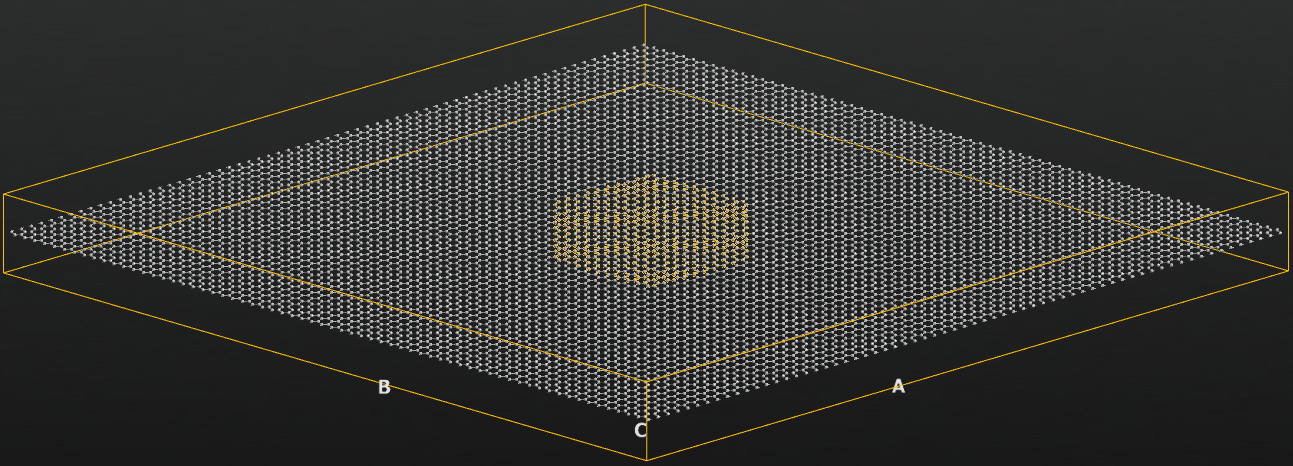
\includegraphics[width=\columnwidth]{Figures/NanoLayer5nm.png}
    \caption{A snapshot from ATK\cite{QuantumWise} showing how the clamped system looks like when at rest. The hexagon in the middle is marked with tags and is the only part of the sheet that is not constrained i.e. the free standing membrane.}
    \label{fig:clamped}

\vspace{0em}

    \centering
    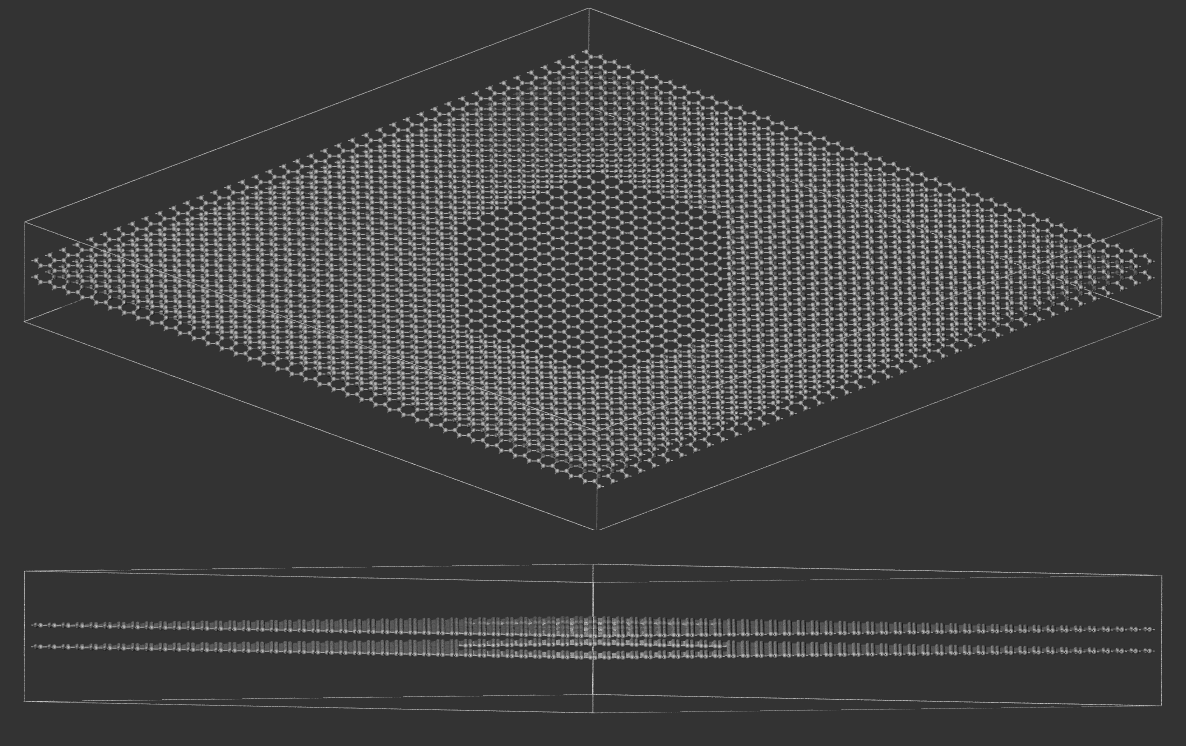
\includegraphics[width=\columnwidth]{Figures/DoubleMembrane.png}
\caption{The picture on top shows the two layer system from above. The one on bottom shows the system from the side. Both snapshots have been taken in ATK\cite{QuantumWise}.}
\label{interlayersys}
\end{figure}
\clearpage
\twocolumngrid

\subsubsection{Frequency vs. membrane size}
In order to find the correlation between frequency of the modes in the membrane and the membrane size, the frequency over each membrane, which varies in size, is extracted and plotted as a function of the size of the given membrane. \\
This is done by defining a sheet of a definite size in VNL and thereafter check the frequencies for the different membranes by inserting the different size membranes, one after the other. The distance from the edge of the membrane, to the edge of the sheet (or the next membrane) is called "neck" and has been chosen to be 5 nm for the biggest membrane which has a 10 nm diameter. With this neck size it is certain that the membrane do not transfer any energy to each other, according to reports \cref{p} \\
Furthermore, only the frequencies for the first couple of modes will be checked. \\
In this section the frequency will sometimes be noted in terms of energy for the modes $[\text{eV}]$. Other times just as the frequency in $[\text{Hz}]$. That is because the energy can be converted to a frequency and vice versa by the relation: $1\text{Hz}=4.13\text{x}10^{-15}\text{eV}$.
\onecolumngrid

\begin{figure}[H]
\centering
\begin{subfigure}{\textwidth}
  \centering
  \vspace{-0.8em}
  \includegraphics[width=1\linewidth]{Figures/FrequencyModeProjectionsNoZoom.eps}
  \label{svfa}
  \vspace{-4.4em}
\end{subfigure}\vspace{1mm}
\begin{subfigure}{\textwidth}
  \centering
  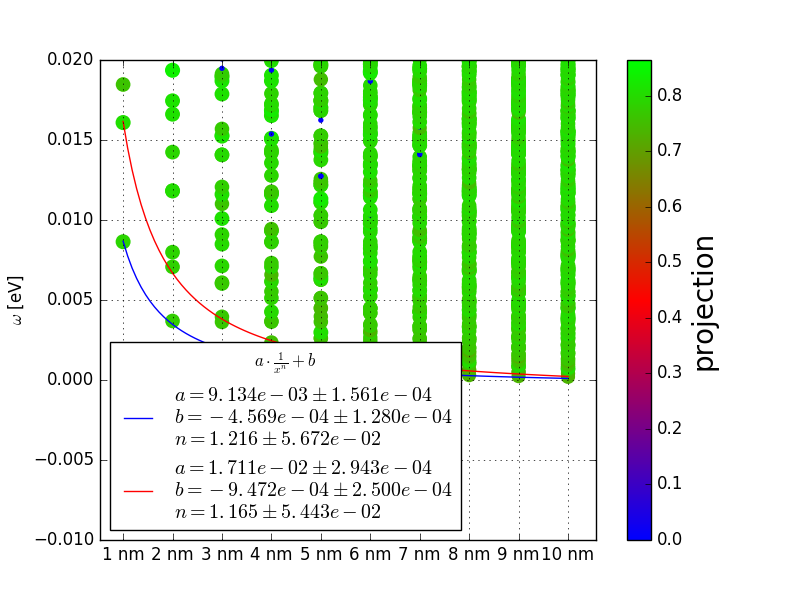
\includegraphics[width=1\linewidth]{Figures/FrequencyModeProjectionsZoomFit.eps}
  \label{svfb}
\end{subfigure}
\vspace{-4em}
\caption{Top: Frequency plotted as a function of membrane size for a one-sheet clamped system. Bottom: Shows the same plot but zoomed in at first three modes. Every green dot being a specific mode, and the red and blue lines being trend curves for the first and second mode}
\label{sizevsfrequency}
\end{figure}
\twocolumngrid

Looking at the data it is clear to see that the frequency decreases when the size of the membrane increase and through our understanding of the physics behind the membrane, the frequency must have the following relation to the membrane size: $f(x)\rightarrow0$ for $x\rightarrow\infty$. Using the regression for the first and second mode it is determined that the relation between frequency and membrane size can be described by:\begin{equation}
    f=a\cdot\dfrac{1}{x^n}
\end{equation}Where $f$ is the frequency, $x$ is the size of the membranes, and where $a$ and $n$ are constants. Comparing the constants for the first mode to the constants for the second it is seen that $a$ relates to the frequency of the first membrane, while $n$ is relatively the same. This indicates that even though the modes start at different frequencies they will conjugate towards zero at the same rate about $\dfrac{1}{x^{1.4}}$. This trend can also be used as a scaling factor to predict the frequency for even bigger membranes, for example: If you want a 20 nm membrane we can predict that the frequency of first mode for this hole will be
    \begin{align}
     f = & \left(8.743\cdot10^{-3}\pm2.012\cdot10^{-4}\right)\nonumber\\
    & \cdot\dfrac{1}{20^{1.428\pm5.166e-4}\text{nm}}\nonumber\\
    = & 1.213\cdot10^{-4}\pm 1.898\cdot 10^{-5} \mathrm{eV}\nonumber\\
    & =29.3\text{GHz}\pm 4.59\text{GHz}
    \end{align}
This prediction fits with our understanding that the phonon in the membrane will decrease and eventually disappear as the membranes gets bigger, but never have a negative frequency.

\subsection{Interlayer interaction}
This section will focus on a simulation of a more realistic system that contains two graphene sheets. See \cref{interlayersys}. One sheet, containing holes, will be constrained and the other sheet will be standing free above. We will test what effect the interaction between the layers will have on the membranes of the free standing sheet. To to this we have chosen a specific holes size for the constrained sheet of 5nm and then varied the strength of the interaction potential between the layer. Three values were chosen: $\epsilon_{graphite}=0.31, \epsilon_{\text{SiO}_{2}}=1.00 \ \text{and} \ \epsilon_{strong}=10.0$. The values are the depth of the potential minimum for graphite, silicon dioxide and then a fictive and very strong potential. The reason for including the very strong potential is to make a reference point for the two other substrate values and how well they correspond with the clamped system.
\onecolumngrid

\begin{figure}[H]
\centering
\begin{subfigure}{0.7\textwidth}
  \centering
  \vspace{-0.8em}
  \includegraphics[width=1\linewidth]{Figures/FrequencyModeProjectionsZetaNoZoom.eps}
  \label{interpota}
  \vspace{-3.8em}
\end{subfigure}\vspace{1mm}
\begin{subfigure}{\textwidth}
  \centering
  \includegraphics[width=1\linewidth]{Figures/FrequencyModeProjectionsZeta.eps}
  \label{interpotb}
\end{subfigure}
\vspace{-4em}
\caption{Top: The figure shows two plots: the small plot to the left shows the lowest modes and their frequencies for the single sheet with a 5nm membrane (shown as green dots).  The plot to the right shows the corresponding modes for the system with two sheets again with a membrane of 5nm, but with three different interaction potentials between the layers: $\epsilon_{graphite}=0.31$, $\epsilon_{\text{SiO}_{2}}=1.00$, $\epsilon_{strong}=10.0$ (from left to right). Bottom: Same plot but zoomed in at the bottom modes. The blue lines indicate the frequency values for the clamped system and shows how much they deviate from the system of two sheets depending on the strength of the potential between the layers.}
\label{interpot}
\end{figure}
\twocolumngrid

As seen on \cref{interpot} there is good correspondence in the frequency values of the clamped system and the two first interaction potentials in the two sheet system. In \cref{freqval}, a list of the frequencies for the two layer system and the deviation of the two layer system with respect to the clamped system can be seen. \cref{freqclamp} shows the frequencies for the clamped system.
% \begin{table}[H]
%   \centering
%   \begin{tabular}{c|c|c|c|c}
%     \toprule
%     Mode & Fq. Clamped $\omega[\text{meV}]$ & Fq. $\epsilon_{graphite}$ $\omega[\text{meV}]$ & Fq. $\epsilon_{SiO_{2}}$ $\omega[\text{meV}]$ & Fq. $\epsilon_{strong}$ $\omega[\text{meV}]$ \\
%     \hline \hline
%     1 & 0.78 & 0.61 & 0.69 & 1.52 \\
%     2 & 1.61 & 1.26 & 1.40 & 2.49 \\
%    4 & 2.61 & 2.10 & 2.35 & 3.81 \\
%    6 & 2.98 & 2.43 & 2.76 & 4.32 \\
%    7 & 3.64 & 2.94 & 3.32 & 4.76 \\
%    \bottomrule
%  \end{tabular}
%  \caption{}
%  \label{freqval}
%\end{table}
%\begin{table}[H]
%  \centering
%  \begin{tabular}{l|r|r|r}
%    \hline
%    Mode & Deviation, graphite & Deviation, Silicon Dioxide & Deviation, Strong \\
%    \hline \hline
%    1 & 21.8\% & 11.5\% & 94.9\%   \\
%    2 & 21.7\% & 13.0\% & 54.7\%   \\
%    4 & 19.5\% & 10.0\% & 46.0\%   \\
%    6 & 18.5\% &  7.5\% & 45.0\%   \\
%    7 & 19.2\% &  8.8\% & 30.8\%   \\
%    \toprule
%    Avg. & 20.2\% & 10.1\% & 54.2\% \\
%    \hline
%  \end{tabular}
%  \caption{}
%  \label{}
%\end{table}
\begin{table}
  \centering
  \begin{tabular}{c|cc}
    \toprule
     Modes &     \multicolumn{2}{c}{Frequency}\\
           &   [\si{\meV}] & [THz] \\
    \hline \hline
           1 &        0.78 & 189 \\
           2 &        1.61 & 389 \\
           4 &        2.61 & 631 \\
           6 &        2.98 & 721 \\
           7 &        3.64 & 880 \\
    \bottomrule
  \end{tabular}
  \caption{Frequencies for modes 1,2,4,6,7 in the clamped system}
  \label{freqclamp}
\end{table}
\begin{table}
  \centering
  \begin{tabular}{cccrr}
    \toprule
              $\epsilon$ & Modes &   \multicolumn{2}{c}{Frequency} & Deviation \\
    $[\SI{8.909}{\meV}]$ &       & [\si{\meV}] & [THz] &      [\%] \\
    \hline \hline
     \multirow{5}*{0.31} &     1 &        0.61 & 147 &    21.8 \\
     \cmidrule(l){2-4}   &     2 &        1.26 & 305 &    21.7 \\
     \cmidrule(l){2-4}   &     4 &        2.10 & 508 &    19.5 \\
     \cmidrule(l){2-4}   &     6 &        2.43 & 588 &    18.5 \\
     \cmidrule(l){2-4}   &     7 &        2.94 & 711 &    19.2 \\
    \midrule
     \multirow{5}*{1.00} &     1 &        0.69 & 167 &    11.5 \\
     \cmidrule(l){2-4}   &     2 &        1.40 & 339 &    13.0 \\
     \cmidrule(l){2-4}   &     4 &        2.35 & 568 &    10.0 \\
     \cmidrule(l){2-4}   &     6 &        2.76 & 667 &     7.5 \\
     \cmidrule(l){2-4}   &     7 &        3.32 & 803 &     8.8 \\
    \midrule
     \multirow{5}*{10.0} &     1 &        1.52 & 368 &   94.9 \\
     \cmidrule(l){2-4}   &     2 &        2.49 & 602 &    54.7 \\
     \cmidrule(l){2-4}   &     4 &        3.81 & 921 &    46.0 \\
     \cmidrule(l){2-4}   &     6 &        4.32 & 1045 &    45.0 \\
     \cmidrule(l){2-4}   &     7 &        4.76 & 1151 &    30.8 \\
    \bottomrule
  \end{tabular}
  \caption{Frequencies for modes 1,2,4,6,7 for the Two layer system with the three potentials $\epsilon_{graphite},\epsilon_{\text{SiO}_{2}},\epsilon_{strong}$ and their deviation from the clamped system}
  \label{freqval}
\end{table}
\begin{table}
  \centering
  \begin{tabular}{cc}
    \toprule
              $\epsilon$ & Average deviation \\
    $[\SI{8.909}{\meV}]$ &              [\%] \\
    \hline \hline
                    0.31 &              20.2 \\
    \midrule
                    1.00 &              10.1 \\
    \midrule
                    10.0 &              54.2 \\
    \bottomrule
  \end{tabular}
  \caption{Table showing the average deviation of the two layer systems with respect to the clamped system}
  \label{}
\end{table}
However, as \cref{interpot} also shows, the projection values does not have as much movement out of the plane as the clamped system. This can possibly be explained by the fact that there is some in-plane movement going on outside the area of the membrane. The calculation sums up movements over the whole sheet, why the out of plane movement over the membrane seems less because of the in-plane movement going on outside the membrane. We will therefore make calculations for the RMS-amplitude of every atom only within the membrane in the clamped system and compare it to corresponding calculations for the two layer system with all three interlayer potentials. \cref{2DRMS} shows the RMS calculations together with the out-of-plane displacements.
\onecolumngrid

\begin{figure}[H]
    \centering
    \includegraphics[width=\columnwidth]{Figures/2DRMS.eps}
    \caption{Figure showing the out of plane displacements with RMS-values for five different modes for the clamped system and the two-layer system with the three different interaction potentials respectively (Top to bottom). The reason why the modes has the values 0,1,3,5,6 is because the modes pairs $[2,3]$, $[4,5]$ are degenerated pairs, why we have only chosen mode 3 and 5.}
    \label{2DRMS}
\end{figure}
\twocolumngrid

In \cref{2DRMS} we can see that there is good correspondence between the clamped system and the two systems with the low interaction potential. Even more so, when looking at the RMS-values we can see that system with the $\text{SiO}_{2}$ ($\epsilon=1.00$). Substrate potential is pretty close to the RMS-values of the clamped system, even closer than graphite. The reason why the system with the strong interaction potential is blue is because the draws the upper sheet down towards the lower one. This causes the area around the rim to be blue no matter what mode we look at. Then again the system with strong interaction potential is only for reference.
\subsection{Modes with varying membranes size, Clamped system}In this section will look at the clamped system only and investigate if and how shape of the modes in the membrane changes as we increase the size of the membrane.
\onecolumngrid

 \begin{figure}
     \centering
     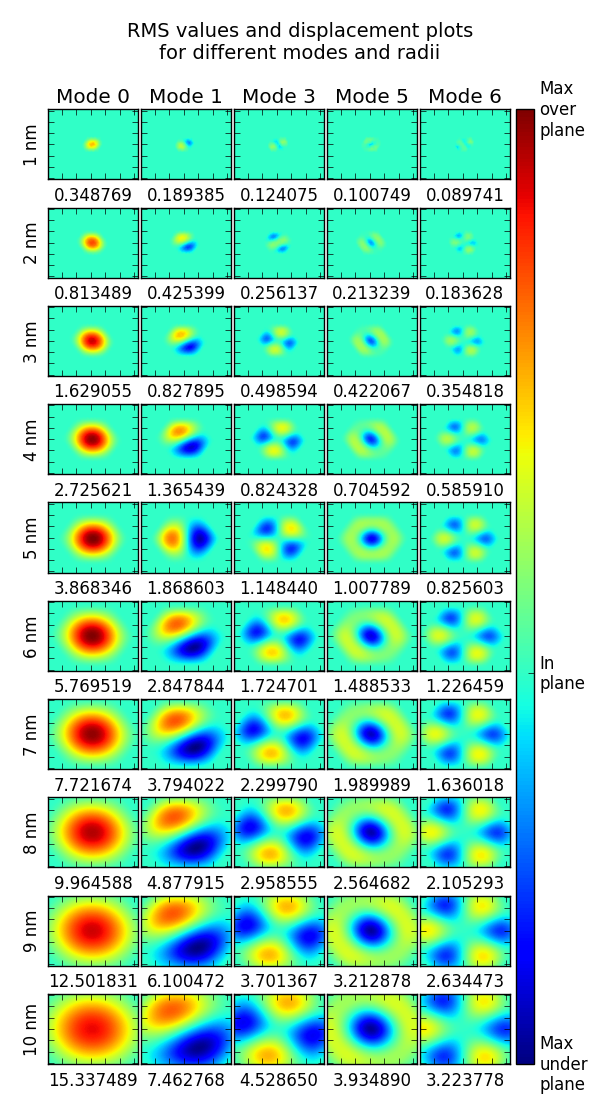
\includegraphics{Figures/2DRMSClamped.eps}
     \caption{Caption}
     \label{BIG}
 \end{figure}
\twocolumngrid

In \cref{BIG} we can see that modes are similar in shape when increasing the membrane size. The size of the modes/membranes change as well as their orientation as some of them rotate around the axis at the center of the membrane going out of the plane. That they change in size, intuitively, makes good sense as we change the size of the membrane itself, but the rotation... When looking at the RMS-values it can also be seen that they increase as the membrane size increase i.e. there is more out of plane movement for larger membranes than small ones. Looking at the modes with respect to RMS, the values decrease as the modes increase. The reason why the RMS increase with the membrane size makes intuitively good sense, the more atoms there is in the membrane the higher the RMS-value. Why the RMS decreases with a mode increase can explained by the fact the an increase in mode number increases the number of nodes in the membrane. The atoms placed at the nodes do not move around that much why their RMS values are close to 0. Looking at \cref{BIG} we can also see that there is more green space i.e. node space as the modes increase no matter the membrane size. In \cref{PLOTZ} there is two plots showing how the RMS-values decrease with the increase of mode numbers for the different hole sizes.
